\newpage

\section{Diagramas de estados}
De forma a ser possível seguir todos os estados do processos principais do fórum, nestes diagramas é pretendido demonstrar o processo de criação de um tópico do fórum por parte de um cliente, o processo de aceder e responder a um tópico privado por parte de um técnico e a autenticação do cliente visto que estas interações são as de maior significância e regradas no software.

\subsection{Diagrama de estados criação de tópico}

Com o diagrama de estados de criação de tópico é pretendido demonstrar o processo de criação de um tópico por parte de um cliente. Assim sendo o cliente primeiramente terá de estar autenticado, caso não esteja este será encaminhado para autenticação. De seguida o cliente criará um novo tópico, após preencher os campos desejados este poderá confirmar o tópico, caso confirme é verificado se o tópico possui título, caso não possua o tópico é invalido pelo que o cliente deverá preencher os dados em falta, caso o título esteja preenchido é verificado se possui descrição, caso não possua é seguido o meso fluxo que o caso anterior, caso contrário é criado um novo tópico. Se o cliente não desejar confirmar o tópico ele poderá cancelar o tópico, quando o assim faz este tópico torna-se cancelado.

\begin{figure}[htb]
    \centering
    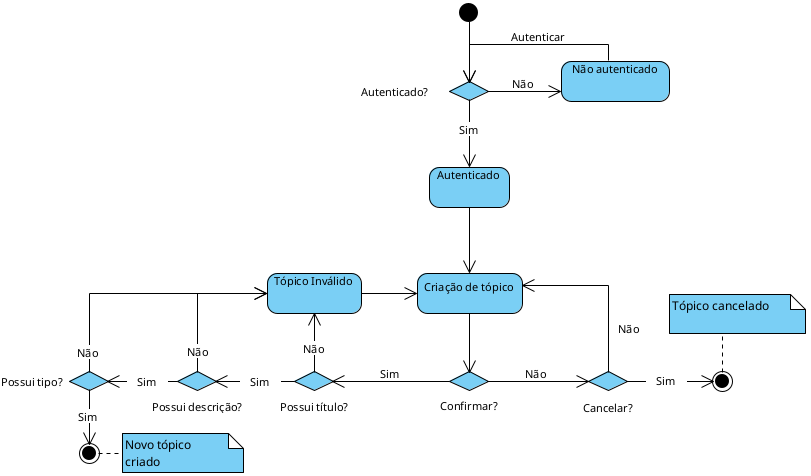
\includegraphics[width=0.9\textwidth]{images/diagramas/estados/criar_topico.png}
    \caption{Diagrama de estados de criar tópico}
    \label{fig:27}
\end{figure}

\newpage

\subsection{Diagrama de estados responder a tópico privado}

Com o diagrama de estados de responder a tópico privado é pretendido demonstrar o processo de seleção e responder a um tópico privado por parte de um técnico. Assim sendo o técnico primeiramente deverá estar autenticado, caso não esteja este será encaminhado para a autenticação. Após a autenticação o técnico estará autenticado e irá por predefinição ver tópicos em destaque, mas visto que se trata de um técnico este poderá ver tópicos privados, nesta listagem este selecionará um tópico ficando assim o tópico selecionado. Assim que o tópico se encontra selecionado o técnico conseguirá responder a este criando um comentário. Após a criação do comentário este poderá confirmar o comentário, caso confirme o comentário ficará criado, caso contrário este comentário ficará cancelado.

\begin{figure}[htb]
    \centering
    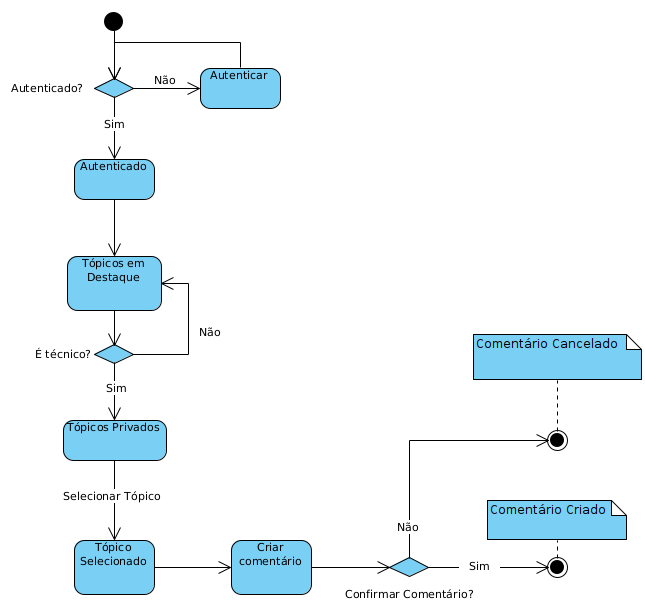
\includegraphics[width=0.7\textwidth]{images/diagramas/estados/responder_topico_tecnico.png}
    \caption{Diagrama de estados de criar tópico}
    \label{fig:28}
\end{figure}

\newpage

\subsection{Diagrama de estados autenticação e validação de conta}

Assim que o cliente decide realizar o login na aplicação este indica as suas credenciais, caso estas credenciais não estejam corretas, a autenticação será incorreta e deverá alterar as credenciais. Caso as credenciais estejam corretas e a conta válida o cliente ficará autenticado, caso contrário o cliente terá uma conta inválida, pelo que a conta deverá ser validada, para  isso o cliente deverá inserir o código de validação da conta, se o código estiver correto, a conta será validada e o cliente ficará autenticado, caso contrário o código será invalido e o cliente deverá indicar o seu código de validação novamente.

\begin{figure}[htb]
    \centering
    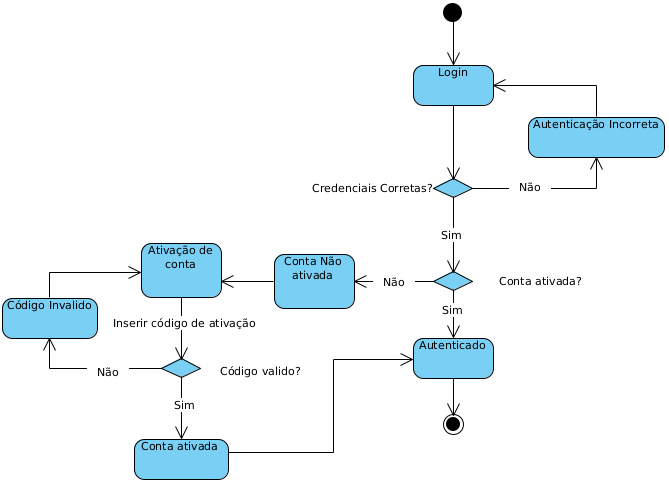
\includegraphics[width=0.7\textwidth]{images/diagramas/estados/autenticacao.png}
    \caption{Diagrama de estados de autenticação e validação de conta}
    \label{fig:29}
\end{figure}
